\section{Test setup}

\subsection{Tools used for testing}

\subsection*{Hardware}
 The platform chosen for test implementation was Nordic Semiconductor nRF52840. The SoC features 2.4 GHz 
 radio and supports a broad variety of wireless protocols. Except for the bare Soc intended to assembly in a 
 custom PCB, the device is manufactured in two main versions: nRF52840 DK, nRF52840 Dongle. Both of them were 
 utilized for the thesis.
 
 Mesh networks were deployed onto the set of 7 nrf52840 DK boards shown in the figure \ref{fig:test_boards}. All of the boards were supplied via USB cables and connected to the workstation.

\begin{figure}[H]
    \centering
    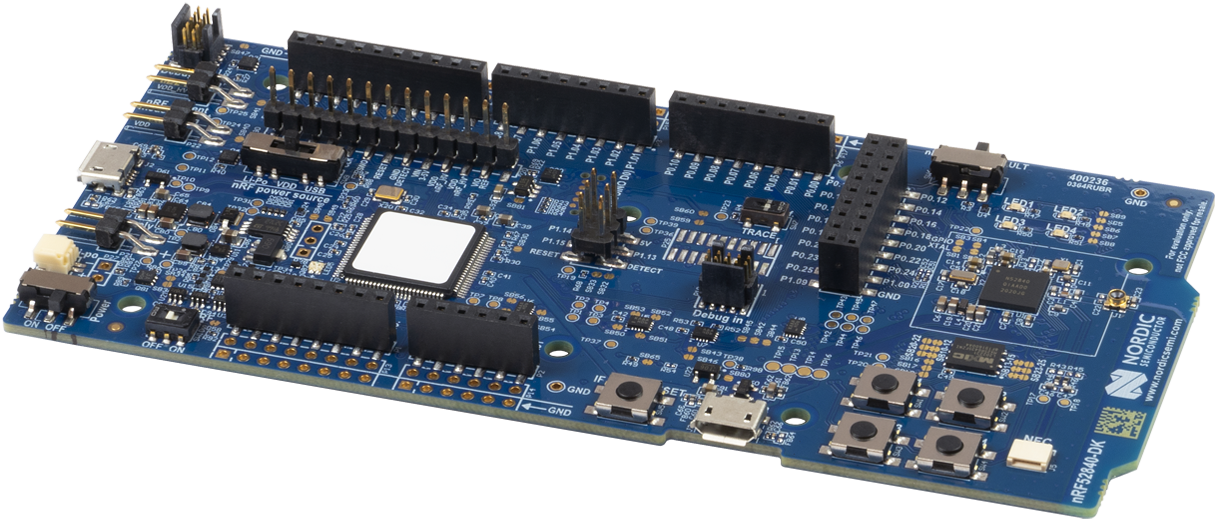
\includegraphics[scale=0.3]{images/test_boards.png}
    \caption{The test setup}
    \label{fig:test_boards}
\end{figure}

\subsection*{Benchmark application}

The most recent implementation of Zigbee and Thread protocols for nRF52840 are released as a components of nRF  
Connect  SDK (abbreviated as \textbf{NCS}). The SDK does not feature any tool which can be used for 
benchmarking Thread and Zigbee. However, such an application existed before- in the previous Nordic Semiconductor SDK (nRF5 SDK for Thread and Zigbee) and was called \textbf{benchmark}. When implementing tests, 
the tool based on 
\textbf{benchmark} was implemented and used to perform tests of a Zigbee network.

\subsection*{Zperf application}

Since Thread protocol is an Internet oriented protocol, an existing methodologies and tools could possibly be used to measure network performance. \textbf{Iperf} is one of the tools specialized in evaluating performance metrics. It was chosen as a basis, because it exists as a sample application for Zephyr RTOS. For this project, the RTT measurement for UDP based connections and support for Thread was added to the original application.

\subsection{Tools used for diagnostics}


\medskip
\section{Performance metrics}

\medskip
\section{Problems encountered}

\medskip
\section{Performance testing}
